\section{Bippit project}
At time of writing I am working over a year in company called \textit{Bippit Ltd}\cite{BIPPIT} on their platform for financial wellbeing. The purpose of the platform is to help users to connect with coaches and to give them tools to educate themselves, get their finances under control and plan for the future.

This project was developed for over 4 years with just handful of developers. Backend is written using Microservices architecture in Rust and there are 2 frontend applications: native iOS and Web. Additionally, there are two other web frontends for management. Admin portal used by advisors for communication with users and by also by support/admin users. Latter is Customer portal, available for our customers (employers) to see interactions of theirs employees with our platform.

\subsection{User journey}
Over the years platform gained a lot of features, so I will highlight just the main ones, to give you some idea of what the platform does. I will describe the flows using User journeys:

\begin{example}[Sign Up]
    Employee Joe of company Z receives an email about gaining access to Bippit platform, because his employer bought it as a benefit. Joe opens up web browser and goes to registration page. He fills email and password and go through the onboarding process (couple of basic questions about his financial experience and goals). Once the registration is completed, he lands on the home page.
\end{example}

\begin{example}[Advisor]
    Right after signUp, Joe is presented with the name of personal financial advisor, who was assigned to him. He can send him a message via chat or preferably book a call, so they can meet face to face, get to know Joe's expectations, look into his finances and set some goals.
\end{example}

\begin{example}[Analyse]
    In the meantime when Joe is waiting for the first meeting with his Advisor, platform offers to connect his bank accounts, so it can show him some insight into his spending. In UK, they have Open banking standard, which allows in just 3 steps give access for application access to his accounts and transactions. After connection is completed, Joe is presented with graphs showing how much in which category he is spending every month. He can also set goals (e.g. wedding or buy a house), connect them with accounts, and it will automatically track any progress (savings).
\end{example}

\begin{example}[Education]
    On Learning page, Joe can read thousands of articles about finances written by our financial Advisors or watch records of past webinars. Also, see any upcoming webinar and register to it.
\end{example}

% \subsection{Vocabulary}
% Before moving into technical side of the thing, we need to first define few terms, which will be used throughout this chapter:
% \begin{description}
%     \item[Insight]
% \end{description}


\subsection{Infrastructure}
Bippit's infrastructure is build on products from HashiCorp (HashiStack). Cloud provider is used for VM provisioning and networking, but they manage the rest by themselves via custom Terraform scripts (IaaS). What are the main components:
\begin{itemize}
    \item \it{Nomad}  is a simple and flexible scheduler and orchestrator to deploy and manage containers. \cite{NOMAD}
    \item \it{Consul} is a service networking solution to automate network configurations, discover services, and enable secure connectivity. \cite{CONSUL}
    \item \it{Vault} secures, stores, and tightly controls access to tokens, passwords, certificates, API keys, and other secrets critical in modern computing. \cite{VAULT}
\end{itemize}

I don't know what was the reason to go with HashiCorp stack, but taking into account experience with it after a year, I am amazed how well the components are integrated and the setup/management of the whole cluster was a breeze in comparisement to Kubernetes (K8s). There are now many managed K8s clusters available, but not a single managed Nomad cluster provider I could find (there was unmanaged.io project, but it does not seem to work anymore). I believe the reason for this is simply - Nomad is just easy to run and manage. I am not condemning K8s, the complexity has for sure it's reason, but just for this project Nomad was more than enough and was much easier to work with. Over the year we had 2 incidents in production. First was caused by some weird state of cluster, which was solved by restarting it and second was caused by our cloud provider, who had networking issues. Since we did not have anyone dedicated for infrastructure and everything was managed by BE developers, we just needed something what is easy to use and will work. Nomad did exactly that without any extra complexity, which we did not need and K8s would most likely add.


\subsection{Microservices}
The whole platform consist of 26 Microservices, 4 of them being backend for frontend. Every microservice exposes its API via HTTP protocol for inter-service communication as well as for outside world, so there is no API Gateway. For background tasks messaging system is used with queues, specifically Amazon's SNS to send messages and SQS to receive them.

Git is used for versioning with repository per Microservice. I see some advantages having repositories separate in compare to Monorepo. Mainly Pull requests are better organized and compact - change to one Microservice should be isolated and having Monorepo allows touching code in multiple Mircoservices, and it would be up to Code reviewer to notice this. Also, it forces developers to think about changes as more isolated since they can modify only single Microservice in single repository - they have to switch to another to do next changes. The same flow could be enforced by for example git hooks, but this way it does not require any configuration. On the other hand, it is a bit harder for newcomers just to download all repositories, since 26 is quite a lot and requires to add some structure to local repositories for easier navigation. However, this is easily mitigated by scripting this process.

% scope and responsibility
Finding the right size of microservices is a hard task. In this project Domain-driver approach was used to locate `small enough parts' (this was approximated) and mapped into Microservices. Some have well-defined boundaries, others some gray zone, few over gowned and should have been split, because maintaining has become much harder with growing complexity. Few examples:

\begin{itemize}
    % TODO add more examples
    \item \it{Financial account} hold bank accounts information for users. Either manually created accounts or those connected.
    \item \it{Transaction} takes care of storing financial transactions.
    \item \it{Categorization} contains pure logic, which categorize transactions into multiple categories.
    \item \it{Orchestrator} is used for scheduled tasks, which trigger complex flows involving multiple microservices for e.g. refreshing cached accounts and transactions from Open Banking and starts following post-processing.
    \item \it{Advisor} was supposed to hold logic and data around advisors and their relation to users. Later on chat functionality were added and since it started with just basic interchange of messages between advisors and users, the unfortunate decision was made to include everything around messaging here as well. Over the time this functionality got extended, and this Microservice has become the most bloated of them all.
\end{itemize}

From examples above is clear, that Microservices have varying scopes/boundaries. Even having the best design possible on the start, over time features are constantly changing and inevitable it leads to uneven distribution of boundaries. It does not mean there is some issue with the design since our system might just be adapting to our changing business requirements, shifts in goals, and our design have to adapt as well. Two outcomes usually might happen. First being proper adaptation to design, once we recognize the change is needed and with it possible refactoring/split/merge of microservices. The second option is what happened to Advisor service. Over time it took more and more features even outside of its scope and when someone recognized the mistake later on the amount of work required to make the necessary changes was just too much to invest at the time.
% how is this possible? Microservice from definition is independent and isolated, so it should be easy just to split into two. Well, even though definitions sound great, the complexity always depends on the actuall implementations. 
% - contracts (swaggers)
% - compatibility
% ability to remove something from contract
% tracking dependency

\subsubsection{Complexity}
% TODO it gets complicated - need to expose lot of APIs (+ maintanance), hard to solve security 
The idea behind having the lot of micro independent services is great from scaling and fast deploy perspective, but as with everything there are also negatives. Every service defines it own interface as in this case as Swagger definition and is kept in sync with code manually, which inevitably leads to problems. Couple of automated solutions exists, which either generates OpenApi definition from the code or the other way around. Unfortunately, it has some limitations, not every language has support for it and I have not seen any project to actually use and fully rely on it. This outdated contracts led to confusion and inability to rely on it. Nowadays for inter-service communication probably gRPC technology would be better, since it has support for every major language and from Schema either server or client implementation can be automatically generated.

Defined contracts either via OpenApi or any other technology needs to be maintained ideally indefinitely, which is off course not possible. Even with the best design in mind, the requirements changes, features get deprecated and maintanance of every outdated/old/not used feature costs a lot of time. In monolithic/modular statically types systems when someone changes interface/contract, the compiler gives instant feedback whether this changes can be made or there are some conflicts and exactly where. In Microservices world, this it is much complex issue. If taken into extreme, every service implements its own client to communication to all dependent micro-services. When this happens as it happened in this project, how one can tell if even one specific change small as removing single field on contract will affect other micro-services if any? Maybe deploying some advances tool for static code analyses for this specific purpose would give some idea, but I doubt it would be reliable. Another option which I have taken after seeing this, also the code duplication with this approach dismal, was to publish client with every change of contract. This way other micro-services simply add client library as dependency instead of implementing its own. Now tracing dependencies between services was simple as to inspect dependencies and look for client libraries. Now at least the non-compatible changes to contracts is at least somehow possible, since new version of client library can be released and every micro-services re-build (e.g. as part of CI) with updated client library to see its affect.

Leveraging code convention across services and dependencies for some static analyses, I was able to generate dependency graph for the whole system, see Graph \ref{img:microservices-current-commented} (something, which was not available and no one paid attention to). This is real-example of what can happen to microservices architecture after 3 years of development and this graph does not include communication via async messages. It is not easy to say whether the state looks bad or not, but I would lean to the bad after seeing the graph. If this was graph of module dependencies of Modulith, it would be take some time do changes, but once done and compiler would be satisfied, it would done. But when someone wants to do these big kind of changes like change contracts (internal just between services) in Microservices it is much more work having to change contract, client implementation, propagate the change into every service where it is used. Just to see where it is used is a task on its own compared to Single process system where every IDE is fully capable to show you in matter of seconds every single usage in codebase. And the worst part being the inability to properly check if all contracts for every service are fully compatible and will work, or if simply there is typo somewhere or during the refactoring one service was simply left out.

\begin{figure}
    \centering
    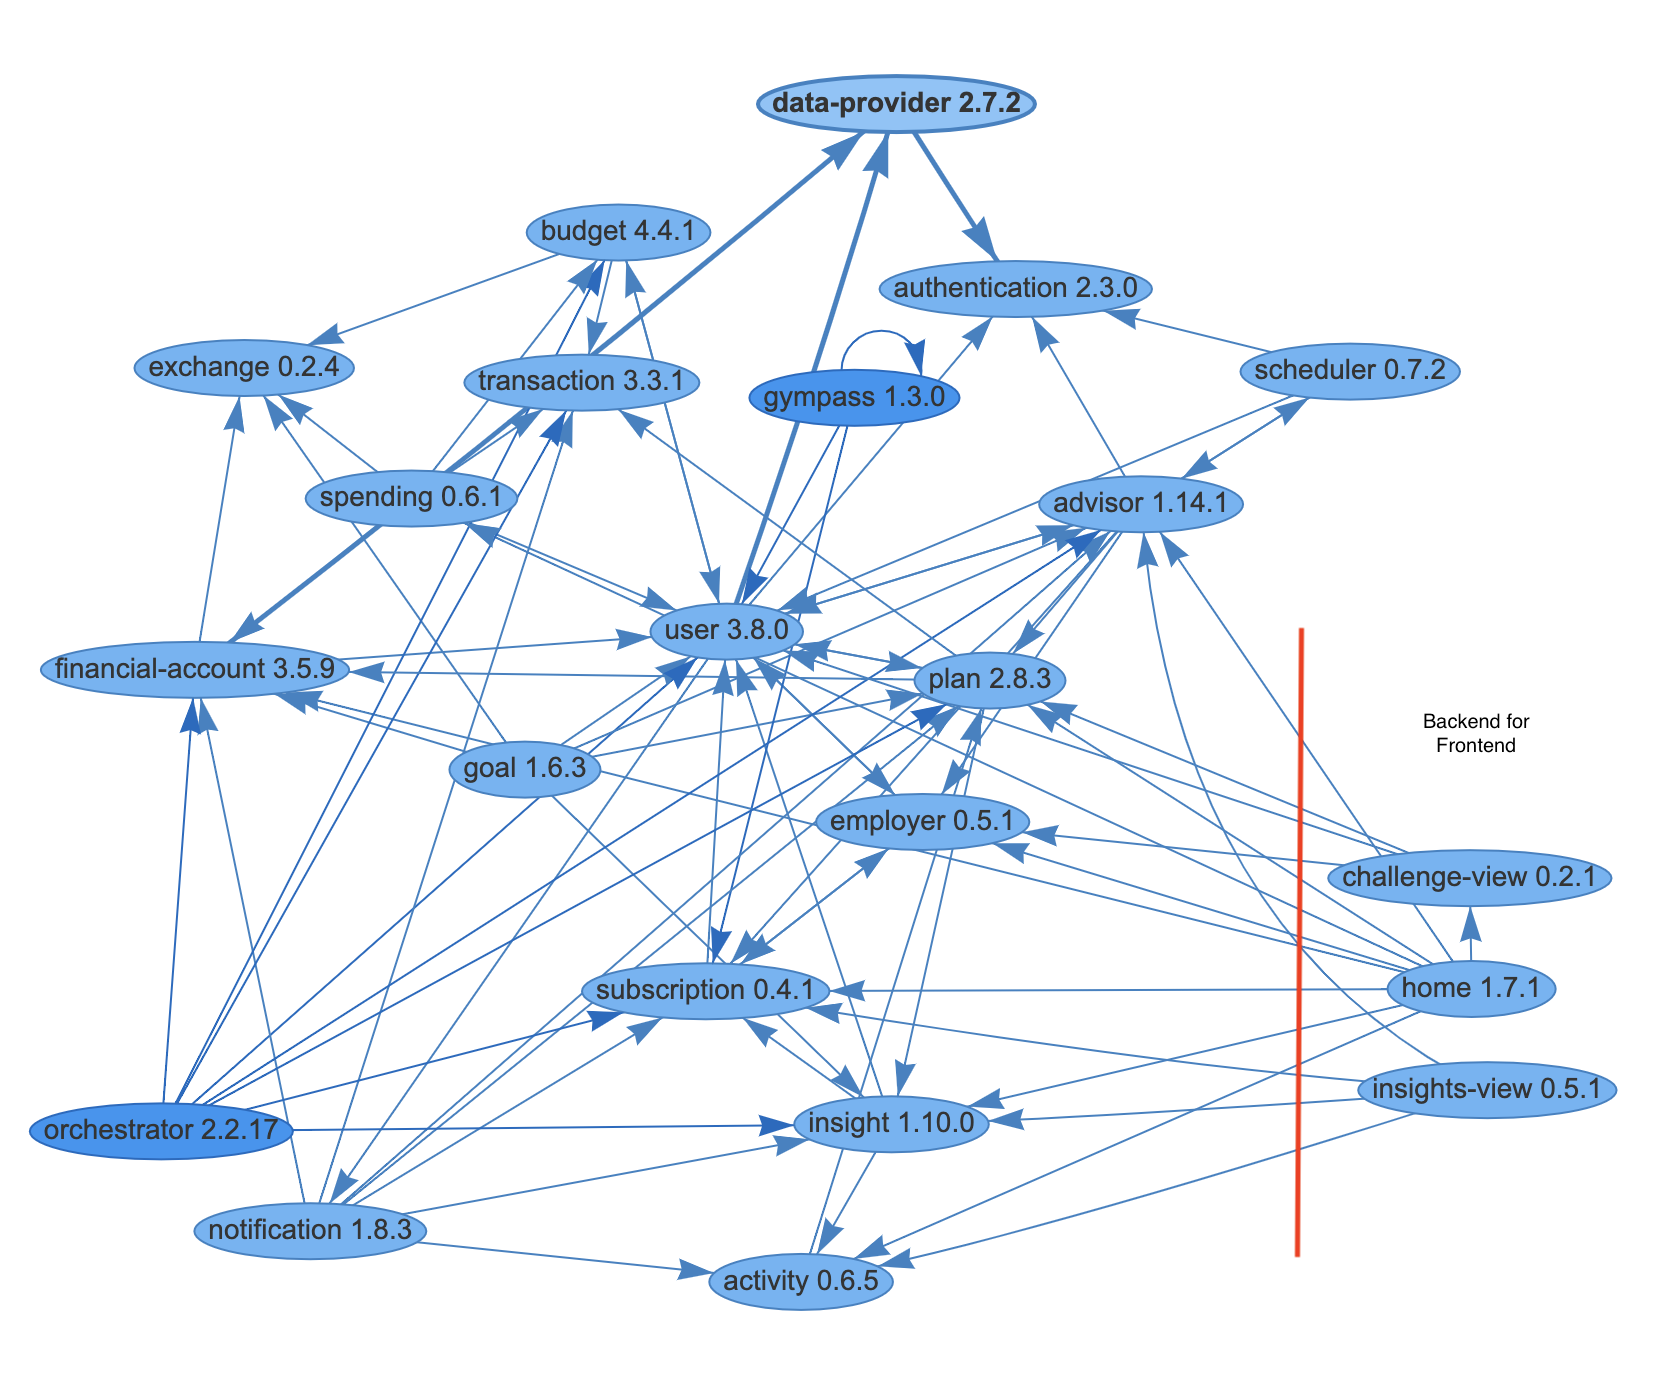
\includegraphics[width=\textwidth]{images/microservices-current-commented.png}
    \caption{Inter microservice dependency graph of Bippit backend after roughly 3 years of development. \label{img:microservices-current-commented}}
\end{figure}

% TODO popsat deployment complexity
% Popsat stroze flow, víc to rezipíšu obecně v Analyse chapter
In terms of performance, there were just two services, which have had noticeable CPU usage and those were processing thousands of financial transactions every time user opened Analyse page, the rest was primarily waiting for database to read or write data. Despite that, we had very linear traffic and every service was just running in two instances without any autoscaling and just few hundred MHz of CPU assigned to it, so it was nearly like Monolith with two instances, with exception even internal requests were load balanced and not just external like with Monolith. So in this case it would easily run even as Monolithic system without any issue with a lot of reserve to grow.

With every bigger feature it meant touching multiple services. Later the deployment required to check all not-deployed work and figuring out what has been tested and can be deployed to production. This flow is most likely the same for all projects, just for Microservices it is easier compared to Monolithic since the change are usually much smaller.